\section{Network Flow II}

We're going to explroe more LP problems today.

\subsection{Bipartite Perfect Matching}
\begin{itemize}
	\item Input: a bipartite (undirected) graph \(G = (L, R, E)\) with \(|L| = |R| = n\) (so each node 
		has a corresponding pair), and want to output a perfect matching from \(L\) to \( R\).

		A perfect matching is one where we can pair every vertex from \(L\) matches with exactly one vertex 
		in \(R\).
	\item Use cases include matching courses and classrooms: you can model a graph where \(L\) denotes 
		the courses and \(R\) are classrooms, and \(E\) denotes whether a classroom can fit a course.  
		So the example of perfect matching is basically asking whether we can assign every course to a classroom.
	\item To solve this, we convert this problem into one of max flow. 
\end{itemize}

\subsubsection{Algorithm}
\begin{itemize}
	\item First copy the graph \(G\) to make \(G'\), and make all the edges directed from \(L\) to \( R\). 
	\item Introduce a source vertex \(s\) that connects to every vertex in \(L\), and introduce a sink 
		that every vertex in  \(R\) connects to. The capacity of each edge will be 1, so this is called 
		``unit flow.''
	\item \textit{Claim:} \(G\) has a perfect matching if and only if the max flow on \(G'\) is \(n\). 
		(intuitively this also makes sense, since had it not been \(n\), then it would mean that 
		some vertex can't be matched)

		\textit{Proof:} First assume that \(G \) has a perfect matching, and let \(M\) denote that perfect 
		matching. We can use this to construct a flow of size \(n\), by putting 1 unit of flow along every 
		edge in \(M\). Then add 1 unit of flow going from \(s\) to every vertex, and add one unit of flow 
		going from every vertex in \(R\) to \(t\). There are \(n\) pairings, so the max flow here is \(n\). 

		First recall from last lecture that if the capacities on our graph are integral, then the max flow is 
		also integral. Now, let \(f\) be an integral flow of size \(n\) in \(G'\). If it's an integral 
		max flow, then we can only assign an integral amount to every edge, and since every edge has capacity 1,
		then our flow basically selects a subset of the edges (since flow is either 0 or 1 along the edges). 

		Each vertex \(u \in L\) alwyas has 1 unit of flow on 1 outgoing edge, since the flow from \(s \to u\)
		is 1, and that flow needs to go somewhere. Similarly, each \(v \in R\) has 1 unit of flow on 1 incoming
		edge. So one vertex in \(u\) has one outgoing edge in \(R\) and one vertex in \(R\) has a 
		corresponding matching in \(L\), so this specifies a matching of size \(n\). 

	\item This is a technique called a \textbf{reduction} from perfect matching to max flow.  
\end{itemize}

\subsection{LP Duality}
\begin{itemize}
	\item Recall that we said last lecture that the max-flow in a graph corresponds to the min-cut on that 
		graph. So we could prove that a flow was optimal by showing a cut of the same value. This idea of 
		correspondence is called \textbf{duality}. 
	\item Suppose we wanted to maximize \(5x_1 + 4x_2\), subject to the constraints:
		\begin{align*}
			2x_1 + x_2 &\le 100\\
			x_1 &\le  30 \\
			x_2 &\le 60\\
			x_1, x_2 &\ge 0
		\end{align*}
		If we were to solve this, we'd get \(x_1 = 20, x_2 = 60\) for a maximum value of 340. (You can 
		check that this is a valid assignment). How do we check 
		that this is the maximum value? Well, we can combine the inequalities in a clever way, which 
		would end up getting us \(5x_1 + 4x_2 \le 340\), which proves that our solution was optimal. 

		To show that this was optimal, we essentially multiplied the inequalities by values \(y_1, y_2, y_3\) 
		that gave us the optimal value. This meant that we were generating the equation:
		\[
			(2y_1 + y_2) x_1 + (y_1 + y_3) x_2 \le 100 y_1 + 30 y_2 + 60 y_3
		\] 
		We want to set \(y_1, y_2, y_3\) such that the LHS is larger than our objective function, while 
		making the RHS as small as possible. Basically, this means that we want to minimize \(100y_1 + 
		30y_2 + 60y_3\) while also requiring that
		\begin{align*}
			0 &\le y_1, y_2, y_3\\
			5 &\le 2y_1 + y_2\\
			4 & \le  y_1 + y_3
		\end{align*}
		So this is basically \textit{another} LP problem! So the original problem is called the \textit{primal
		LP}, and the second one is called the \textit{dual LP}. Because of the way we set this up 
		(with the maximization/minimization), it guarantees that any satsifying assignment of the 
		primal LP will be less than that of the dual LP. This is the \textit{magic trick}: the fact that we can 
		always convert any maximization LP into a minimization in the dual LP. 

		\comment{Turns out that if we take the dual twice, we get back the original LP.}
	\item This is a fairly standard exam problem: given a primal LP, compute the dual.   
	\item There is also a matrix representation of the same problem. Recall the standard form for expressing
		LPs as maximizing \(c^\top \vec x\) subject to the constraints given by 
		\(A \cdot \vec x \le \vec b\) and \(\vec x \ge 0\). 
	\item To construct the dual, we want to minimize 
		the quantity \(\vec b^\top \cdot \vec y\), where \(b\) used to be the constraints earlier. Our 
		constraints are given by \(A^\top \cdot \vec y \ge \vec c\) and \(\vec y \ge 0\)
	\item The theorem we saw earlier is called \textbf{weak duality}, which says that all feasible 
		solutions \(x\) to the primal LP are less than the solutions \(y\) to the dual LP. The proof 
		is as follows:

		The primal LP maximization is written as \(\vec c^\top x\), but we know that \(\vec c\) has another 
		representation as \(A^\top \vec y\), so we can write: 
		\[
		\vec c^\top \vec x \le (\vec y^\top A )\vec x \le y^\top b
		\] 
		Then, since \(y^\top b = b^\top y\), then we have the inequality \(c^\top x \le b^\top y\). 
	\item Graphically we can visualize this as:
		\begin{center}
			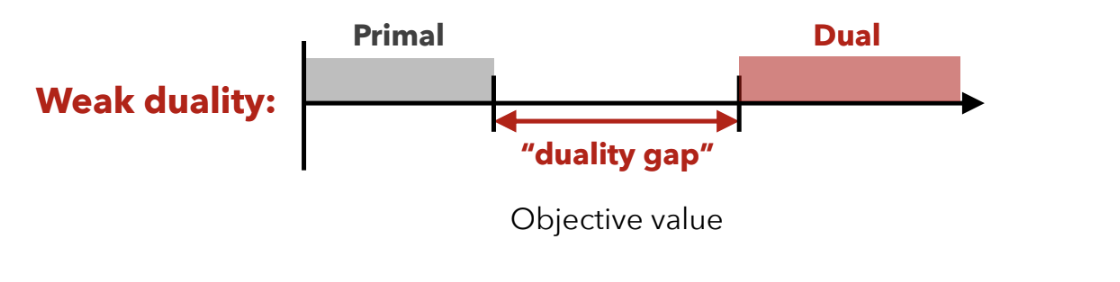
\includegraphics[scale=0.7]{LP-duality-gap.png}
		\end{center}
	\item \textit{Theorem:} If the primal LP is bounded (by any number), 
		then the optimal solution to the 
		Primal LP is equal to that of the dual LP. So in this case, the duality gap is 0 

		\question{Doesn't this apply to most cases?}
	\item The max-flow min-cut principle we had earlier is an example of an LP problem and a corresponding
		dual. So another way of proving what we did was to show that the min cut can also be written as a 
		LP. Then, we can show that they are the duals of each other, and since the max-flow problem is 
		always bounded, then we know that the optimal solution is when they are equal by strong duality. 
\end{itemize}
\subsection{Zero-Sum Games}
\begin{itemize}
	\item Input: a ``payoff'' matrix \(M\), and two players: a row and column player. 
	\item The matrix \(M\) specifies the amount that the row player wins, and the column specifies how much 
		the column player wins. An example of this is rock paper scissors:
		\begin{center}
			\begin{tabular}{c|c|c|c}
				& Rock & Paper & Scissors\\
				\hline
				Rock & 0 & -1 & 1\\
				\hline 
				Paper & 1 & 0 & -1\\
				\hline
				Scissors & -1 & 1 & 0
			\end{tabular}
		\end{center}
	\item In general, the row player selects a row \(r\) and the column player picks a column \(c\). Then, 
		we say that the row player wins \(M_{r, c}\), while the column player wins \(-M_{r, c}\).
	\item This is a zero-sum game because the sum of every row and column is 0. 
	\item There are two strategies the players are allowed: 
		\begin{itemize}
			\item Pure strategy: pick one row/column and play their selection (e.g. row player always picks rock)
			\item Mixed strategy: a probability distribution over pure strategies (e.g. we can have
				\(P[\text{rock}] = 
				\frac{1}{3}, P[\text{paper}] = \frac{1}{3}, P[\text{scissors}] = \frac{1}{3}\) ) 

				Also notice that the average score across all these strategies is 0, no matter what the column
				player does.
		\end{itemize}
\end{itemize}
\subsubsection{Game 1}
\begin{itemize}
	\item The game is described as:
		\begin{center}
			\begin{tabular}{c|c|c}
				& P1 & P2\\
				\hline
				P1 & 3 & -1\\
				\hline
				P2 & -2 & 1
			\end{tabular}
		\end{center}
	\item We want the row player to announce their strategy first, then the column player announces their 
		strategy second. Because this is slightly unfair to the row player, we let the row player 
		announce a mixed strategy \(P = (p_1, p_2)\) where \(p_i\) is the probability that row \(i\) is chosen. 
	\item The column player will respond by choosing a mixed strategy of their own, with 
		distribution \(Q = (q_1, q_2)\) where $q_i$ is the probability of choosing row \(i\). 
	\item Then, the row player's average score is \(S(p, q)\) is the expected value that they get. So in 
		this case:
		\[
		S(p, q) = 3p_1q_1 - p_1q_2 - 2p_2q_1 + p_2q_2
		\] 
		So, the column player's best strategy is to minimize \(S(p, q)\), while the row player wants 
		to maximize \(S(p, q)\).
	\item For the column player, they will choose the best strategy for themselves, after having seen \(p\). 
		So, since the column player knows what \(p\) the row player chose, then their minimization is the 
		same as just minimizing over pure strategies:
		\[
			\min_{\text{mixed strategies}} \{S(p, q)\} = \min_{\text{pure strategies}} 
			\{3p_1 - 2p_2, p_2 - p_1\} 
		\]
	\item The row player goes first, so their strategy is that they would want to maximize the 
		column player's response. So for them they want to compute:
		\[
			\max_{\text{mixed strategies}} \{\min \{3p_1 - 2p_2, p_2 - p_1\} \} 
		\] 
	\item We'll see next time that this is exactly the same as computing two LPs, which are duals of each other!
\end{itemize}
